% CVPR 2022 Paper Template
% based on the CVPR template provided by Ming-Ming Cheng (https://github.com/MCG-NKU/CVPR_Template)
% modified and extended by Stefan Roth (stefan.roth@NOSPAMtu-darmstadt.de)

\documentclass[10pt,twocolumn,letterpaper]{article}

%%%%%%%%% PAPER TYPE  - PLEASE UPDATE FOR FINAL VERSION
%\usepackage[review]{cvpr}      % To produce the REVIEW version
\usepackage{cvpr}              % To produce the CAMERA-READY version
%\usepackage[pagenumbers]{cvpr} % To force page numbers, e.g. for an arXiv version

% Include other packages here, before hyperref.
\usepackage{graphicx}
\usepackage{amsmath}
\usepackage{amssymb}
\usepackage{booktabs}
\usepackage[export]{adjustbox}
\usepackage{multirow}


% It is strongly recommended to use hyperref, especially for the review version.
% hyperref with option pagebackref eases the reviewers' job.
% Please disable hyperref *only* if you encounter grave issues, e.g. with the
% file validation for the camera-ready version.
%
% If you comment hyperref and then uncomment it, you should delete
% ReviewTempalte.aux before re-running LaTeX.
% (Or just hit 'q' on the first LaTeX run, let it finish, and you
%  should be clear).
\usepackage[pagebackref,breaklinks,colorlinks]{hyperref}


% Support for easy cross-referencing
\usepackage[capitalize]{cleveref}
\crefname{section}{Sec.}{Secs.}
\Crefname{section}{Section}{Sections}
\Crefname{table}{Table}{Tables}
\crefname{table}{Tab.}{Tabs.}


%%%%%%%%% PAPER ID  - PLEASE UPDATE
\def\cvprPaperID{*****} % *** Enter the CVPR Paper ID here
\def\confName{CVPR}
\def\confYear{2022}


\begin{document}

%%%%%%%%% TITLE - PLEASE UPDATE
\title{Open-Set Domain Adaptation through Self-Supervision}

\author{Daniele Rege Cambrin, Kylie Bedwell, Tommaso Natta, Ehsan Ansari Nejad\\
Politecnico di Torino\\
Corso Duca degli Abruzzi, 24\\
10129 Torino, ITALY\\
{\tt\small s290144@studenti.polito.it, s287581@studenti.polito.it} \\
{\tt\small s282478@studenti.polito.it, s288903@studenti.polito.it}
% For a paper whose authors are all at the same institution,
% omit the following lines up until the closing ``}''.
% Additional authors and addresses can be added with ``\and'',
% just like the second author.
% To save space, use either the email address or home page, not both
}
\maketitle

%%%%%%%%% ABSTRACT
\begin{abstract}
Large amounts of data are available for use in computer vision research however the costs of labeling the data is high. Self-supervision techniques can be used to address this problem. This study investigates the use of self-supervision in an open-set domain adaptation scenario. A self-supervised tasks is trained alongside a classification task to separate known classes from unknown classes in the target domain. The technique investigated was a simplification of the Rotation-based Open Set (ROS) method, and was found to be less accurate but applicable to simplified scenarios. Various self-supervised tasks were also compared and the rotation recognition task was found to be the most robust compared to horizontal flipping or solving jigsaw puzzles. The inclusion of center loss during training was also investigated but the results were deemed inconclusive.
\end{abstract}

%%%%%%%%% BODY TEXT
\section{Introduction}
\label{sec:intro}

In the computer vision research area large amounts of unlabeled data are available, however the cost of labeling this data is high ~\cite{Csurka2017, Zhang2016}. Domain adaptation is one technique that can be used to exploit the unlabeled data by first training a model on labeled data from a different but similar domain (the \textit{source} domain), and then applying this model to the unlabeled data ( the \textit{target} domain). This technique assumes the distribution of both source and target domains are similar and describe the same class labels, also known as the \textit{closed-set} scenario~\cite{Bucci2020}. When applied to real-word scenarios however it is possible that the target domain includes previously unseen classes, known as the \textit{open-set} scenario. These extra class labels in the target domain will cause performance degradation of the classification model and should be identified and isolated. The problem thus consists of two steps: first separating the target domain into known and unknown samples; then conducting domain alignment between the source domain and the known samples of the target domain. 

Self-supervised learning can be used to separate the known class samples in the target domain from the unknown samples. Self-supervised learning involves the transformation of data using a known transform (for example by using image rotation), then training a model to predict the transformation~\cite{Xu2019}. When used in an object classification task and considering the image rotation transformation, the correct orientation of an object is domain-invariant. In this way the model can be trained to predict the correct orientation of the image using data from the source domain, then applied to the images of the target domain. If the orientation of a sample in the target domain is predicted correctly then it is considered to be of a \textit{known} class. Contrarily if the orientation is not prediction correctly it is labelled as \textit{unknown}. 

Domain adaptation can then be performed between the samples in the source domain and the samples recognized as known in the target domain. When applying domain adaptation to an open-set scenario (Open-Set Domain Adaptation or OSDA) the samples classified as unknown can be treated as a separate class and incorporated into the Closed-Set Domain Adaptation (CSDA) task~\cite{Pau2020}. The self-supervised rotation task can also be used to reduce the domain shift during this step, using the Rotation-based Open Set (ROS) method developed by Bucci \etal \cite{Bucci2020}.

This study investigates the use of a simplified ROS method for object classification on the \textit{Office-Home} dataset \cite{OfficeHome}. Alternative self-supervised tasks as well as the inclusion of center loss are also considered and their performance on the object classification task is evaluated.


%------------------------------------------------------------------------
\section{Related Work}
\label{sec:relatedWork}

\textbf{Anomaly detection}, or outlier/novelty detection, in an open-set scenario can be used to detect samples belonging to the unknown or unseen class. Various different approaches for anomaly detection have been used in the literature as applied to the open-set scenario. Golan and El-Yanic \cite{Golan2018} present a method for using geometric transformations to create a self-labeled dataset. In this way the neural classifier learns features that are effective for the detection of anomalies.  Sakurada and Yairi \cite{Sakurada2014} on the other hand make use of auto-encoders with dimensionality reduction. This method assumes the data have correlations that can clearly separate normal and anomalous samples when reduced to a lower dimensional subspace. After the test data is projected into the subspace it is then reconstructed and the corresponding reconstruction error is used to identify the anomalous samples.


\textbf{Self-supervised learning} has been a key concept aimed at reducing the need for human labeling of data. It has also created opportunities for the use of data in problems where supervision is not possible \cite{Yaman2020}. Self-supervised learning consists of choosing a self-supervised task (or pretext task) to train alongside the main classification task. One possible self-supervised task is image rotation prediction, which is reported to perform best for visual representation learning \cite{Xu2019, Gidaris2018}. However many options are available, including image-patch based methods \cite{Mundhenk2018, Kim2018}, horizontal flipping \cite{Golan2018}, or by solving jigsaw puzzles \cite{Carlucci2019, Kim2018}. 


\textbf{Domain adaptation} techniques have advanced significantly in recent years for the closed-set scenario \cite{Pau2020}, however for real-world applications the closed-set assumption is often not applicable \cite{Ren2021}. It has become increasingly important to develop robust techniques for open-set domain adaptation to address this problem. Recent studies in this field include: the development of a generic approach to learn a linear mapping between the features of the source domain and target domain \cite{Pau2020}; the use of self-supervision to improve the generalization of models to different domains \cite{Carlucci2019}; partial domain adaptation by using a discrepancy criterion to partially align features whilst avoiding negative transfer \cite{Ren2021}. These techniques have been reported to perform well, and increase the applicability of domain adaptation methods to real-world applications \cite{Carlucci2019, Ren2021,Pau2020}.


\textbf{Rotation-based Open Set} (ROS) is a specific technique developed by Bucci \etal \cite{Bucci2020}. ROS is a two-stage method for open-set domain adaptation. The first stage separates samples in the target domain into known and unknown categories by training the model on a multi-rotation recognition task. The rotation recognition task includes the use of the center loss to improve performance by learning a center of the features and minimizing the distances between features and their corresponding centers \cite{Wen2016}. The second stage conducts domain alignment, training both semantic and rotation classifiers to classify known target samples. Bucci \etal \cite{Bucci2020} also propose the use of the harmonic mean of the average class accuracies  for the known and unknown classes as a more robust and balanced evaluation metric.


%------------------------------------------------------------------------
\section{Method}
\label{sec:method}

This study aims to solve the open-set scenario by using self-supervised learning with domain adaptation. Image rotation recognition has been chosen as the self-supervised task due to it's good performance for visual representation learning \cite{Xu2019, Gidaris2018}. The rotation recognition task involves taking the original image sample from the source domain and rotating it clockwise a set amount (for example by 0$^{\circ}$, 90$^{\circ}$, 180$^{\circ}$ or 270$^{\circ}$). A rotation classifier is then trained to predict the correct orientation of the object. The correct orientation of the object, however, is not an inherent property of an image, for example consider the pens in Figure \ref{fig:RotatedPens}. When analyzing a rotated image of a pen it is not possible to infer the original rotation. The original image is therefore included in the rotation classifier and the relative rotation analysed instead. In training the rotation classifier the features of the original sample are concatenated with the features of the rotated sample. By including the original samples the network is also able to learn features that are more discriminative between class labels, focusing more on the shape of the object and less on the texture \cite{Bucci2020}, as shown in Figure \ref{fig:RotationFeatures}.

\begin{figure}[!htb]
  \centering
   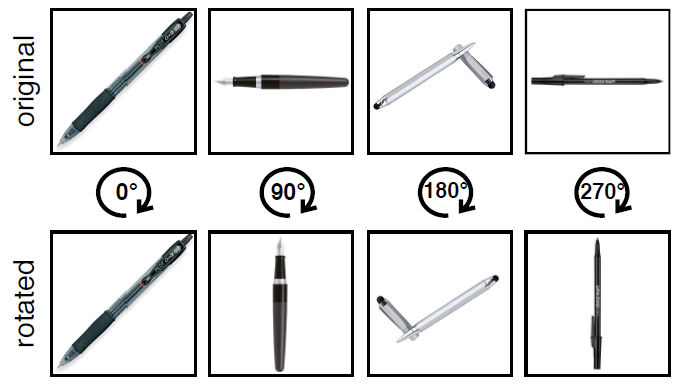
\includegraphics[width=0.9\linewidth]{Figures/RotatedPens.png}
   \caption{Relative orientations of pens with respect to the original images \cite{Bucci2020}.}
   \label{fig:RotatedPens}
\end{figure}

\begin{figure}[!htb]
  \centering
   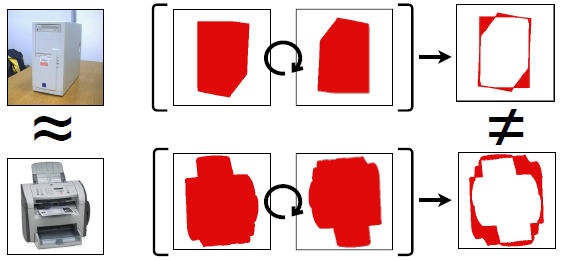
\includegraphics[width=0.9\linewidth]{Figures/RotationFeatures.png}
   \caption{Image rotations help the network learn features that discriminate the shape of objects \cite{Bucci2020}.}
   \label{fig:RotationFeatures}
\end{figure}

To solve the open-set domain adaptation problem a simplified version of the ROS method (Figure \ref{fig:ROS}) is used. This version uses a single-head rotation classifier and does not include the center loss, however the effect of the center loss is evaluated subsequently as a variation to this method. Alternative self-supervised tasks are also considered, including horizontal flipping and through solving jigsaw puzzles. These variations are analyzed in Section \ref{sec:variations}.

\begin{figure*}[!htb]
  \centering
   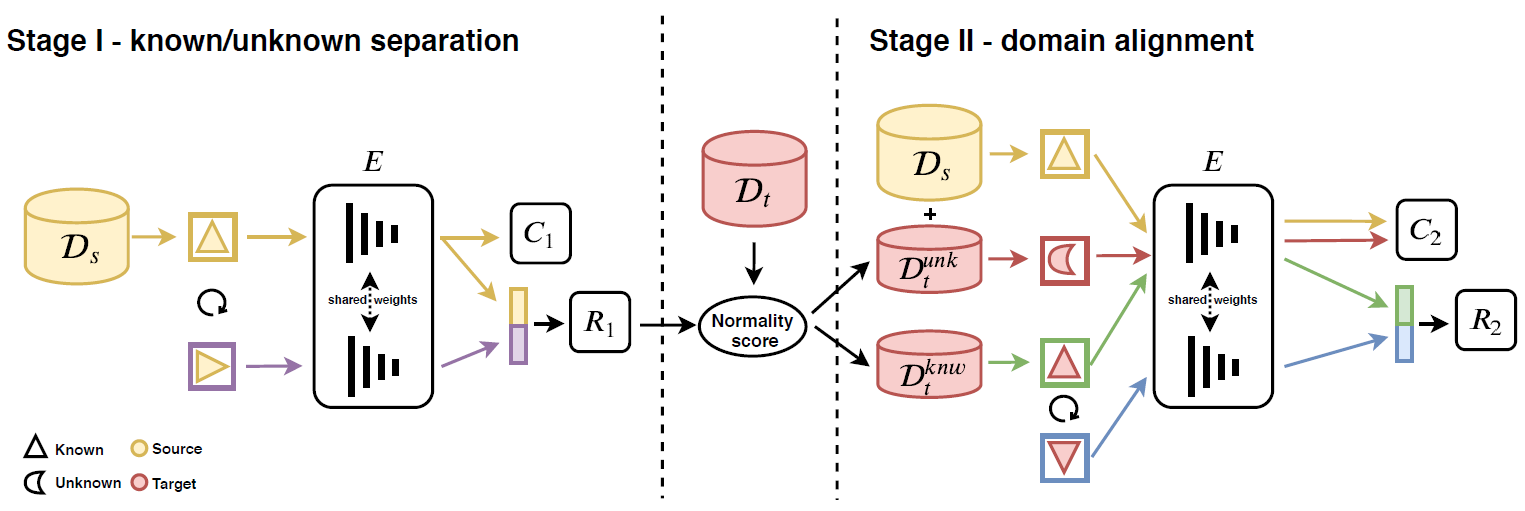
\includegraphics[width=0.9\linewidth]{Figures/ROS.png}
   \caption{Rotation-based Open Set (ROS) method schematic illustration \cite{Bucci2020}.}
   \label{fig:ROS}
\end{figure*}

\subsection{Stage I - known/unknown separation}

Stage 1 of the simplified ROS method involves training both an object classifier and a rotation recognition task on data from the source domain, as shown on the left side of Figure \ref{fig:ROS}, where $D_s$ is the source domain dataset, $E$ is the encoder, $C_1$ is the object classifier and $R_1$ is the rotation classifier. The object prediction is based on the features of the original source samples, whereas the rotation prediction is based on the concatenated features of the original and rotated samples. The object classification and rotation recognition tasks are trained simultaneously to minimize the total loss objective function given by:
\begin{equation}
  L_{tot} = L_{cls} + \alpha_1 L_{rot} ,
  \label{eq:totalloss}
\end{equation}
where $L_{cls}$ is the loss from the object classifier, $L_{rot}$ is the loss from the rotation classifier, and $\alpha_1$ is the weight assigned to the rotation recognition task. The value of $\alpha_1$ is tuned according to the performance of the network, as detailed in Section \ref{sec:ablation}.


\subsubsection*{Target evaluation}

Once the rotation classifier has been well trained it can be used to identify the known classes of the target domain, and separate these samples from the unknown classes. The method is illustrated in the center of Figure \ref{fig:ROS}, where $D_t$ is the target domain dataset, $D_t^{unk}$ is the dataset of target samples identified as belonging to an unknown class, and $D^{knw}_t$ is the dataset of target samples identified as belonging to a known class. The rotation classifier is applied to each of the target samples and generates a score for each of the possible rotations. The normality score is then computed as the rotation with the maximum score (highest prediction).

The precision of the normality score is then evaluated using the AUC (area under receiver operating characteristics (ROC) curve) metric. The AUC metric reduces analysis of the ROC curve to a single scalar value which can be used to compare the performance of classifiers \cite{Fawcett2006}. The higher the AUC score the better the classifier overall, with scores $> 0.5$ showing an improvement over random guessing.

If the AUC is $> 0.5$ then the normality score can be used to conduct the known/unknown separation subject to a selected threshold, i.e. if the normality score is above the threshold the sample is considered as known and added to $D^{knw}_t$, otherwise it is considered as unknown and added to $D_t^{unk}$. The threshold value is also tuned according to the performance of the network, as detailed in Section \ref{sec:ablation}.


\subsection{Stage II - domain alignment}
\label{sec:stage2}

In stage 2 of the simplified ROS method the unknown dataset created from the target domain $D_t^{unk}$ is combined with the samples from the source domain $D_s$, with the unknown samples representing an additional `unknown' class. The object classifier $C_2$ is thus trained to recognize samples belonging to the unknown class. Concurrently, the known target samples  $D^{knw}_t$ are used for the source-target adaptation by training the rotation recognition task $R_2$. The method is shown on the right side of Figure \ref{fig:ROS}. As in stage I, the object classification and rotation recognition tasks are trained simultaneously to minimize the total loss objective function given by:
\begin{equation}
  L_{tot} = L_{cls} + \alpha_2 L_{rot} ,
  \label{eq:totalloss}
\end{equation}
where $\alpha_2$ is the weight assigned to the rotation recognition task of stage 2. The value of $\alpha_2$ is also selected to provide the best performance, detailed further in Section \ref{sec:ablation}. 


\subsubsection*{Final evaluation}

Once the classifiers have been trained the final evaluation can be completed. Three metrics are considered for the evaluation: the accuracy of the object classifier in correctly classifying objects of the known category $OS^*$; the accuracy of the object classifier in correctly identifying objects of the unknown category $UNK$; and the harmonic mean $HOS$ between the two accuracies $OS^*$ and $UNK$, as defined in \cite{Bucci2020}. The harmonic mean is calculated as:
\begin{equation}
 HOS = 2\, \frac{OS^* \times UNK}{OS^* + UNK} ,
 \label{eq:hos}
\end{equation}
and provides a balanced measure of performance of the classifier at recognizing both known and unknown samples.


%------------------------------------------------------------------------
\section{Experiments}
\label{sec:experiments}

The proposed method was tested on the \textit{Office-Home} dataset \cite{OfficeHome}. This dataset consists of four separate domains for image classification: Art, Clipart, Product and Real World. An example of the difference between images in these domains is shown in Figure \ref{fig:domains}. For this experiment each domain included two sets of images, one when behaving as the source domain and another as the target. The dataset contained 65 classes in total.  The classes were sorted alphabetically and the first 45 classes were treated as known and formed the list of images for the source domain, the remaining 20 were considered unknown and included in the list of images for the domain when behaving as the target domain.

\begin{figure}[!htbp]
  \centering
  \begin{adjustbox}{minipage=\linewidth,scale=0.8}
  \begin{subfigure}[b]{0.45\columnwidth}
    \centering
    
\includegraphics[width=\linewidth]{Figures/Art_Radio.jpg}
    \caption{Art}
    \label{fig:short-a}
  \end{subfigure}
  \hfill
  \begin{subfigure}[b]{0.45\columnwidth}
\centering
    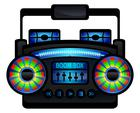
\includegraphics[width=\linewidth]{Figures/Clipart_Radio.jpg}
    \caption{Clipart}
    \label{fig:short-b}
  \end{subfigure}
\vskip\baselineskip
  \begin{subfigure}[b]{0.45\columnwidth}
\centering
    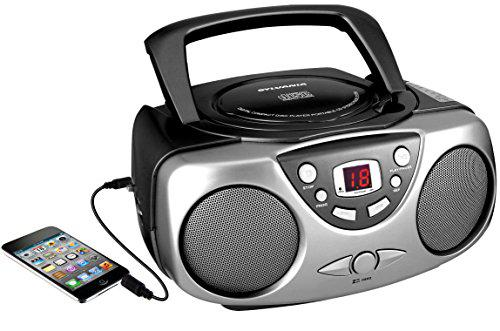
\includegraphics[width=\linewidth]{Figures/Product_Radio.jpg}
    \caption{Product}
    \label{fig:short-c}
  \end{subfigure}
  \hfill
  \begin{subfigure}[b]{0.45\columnwidth}
\centering
    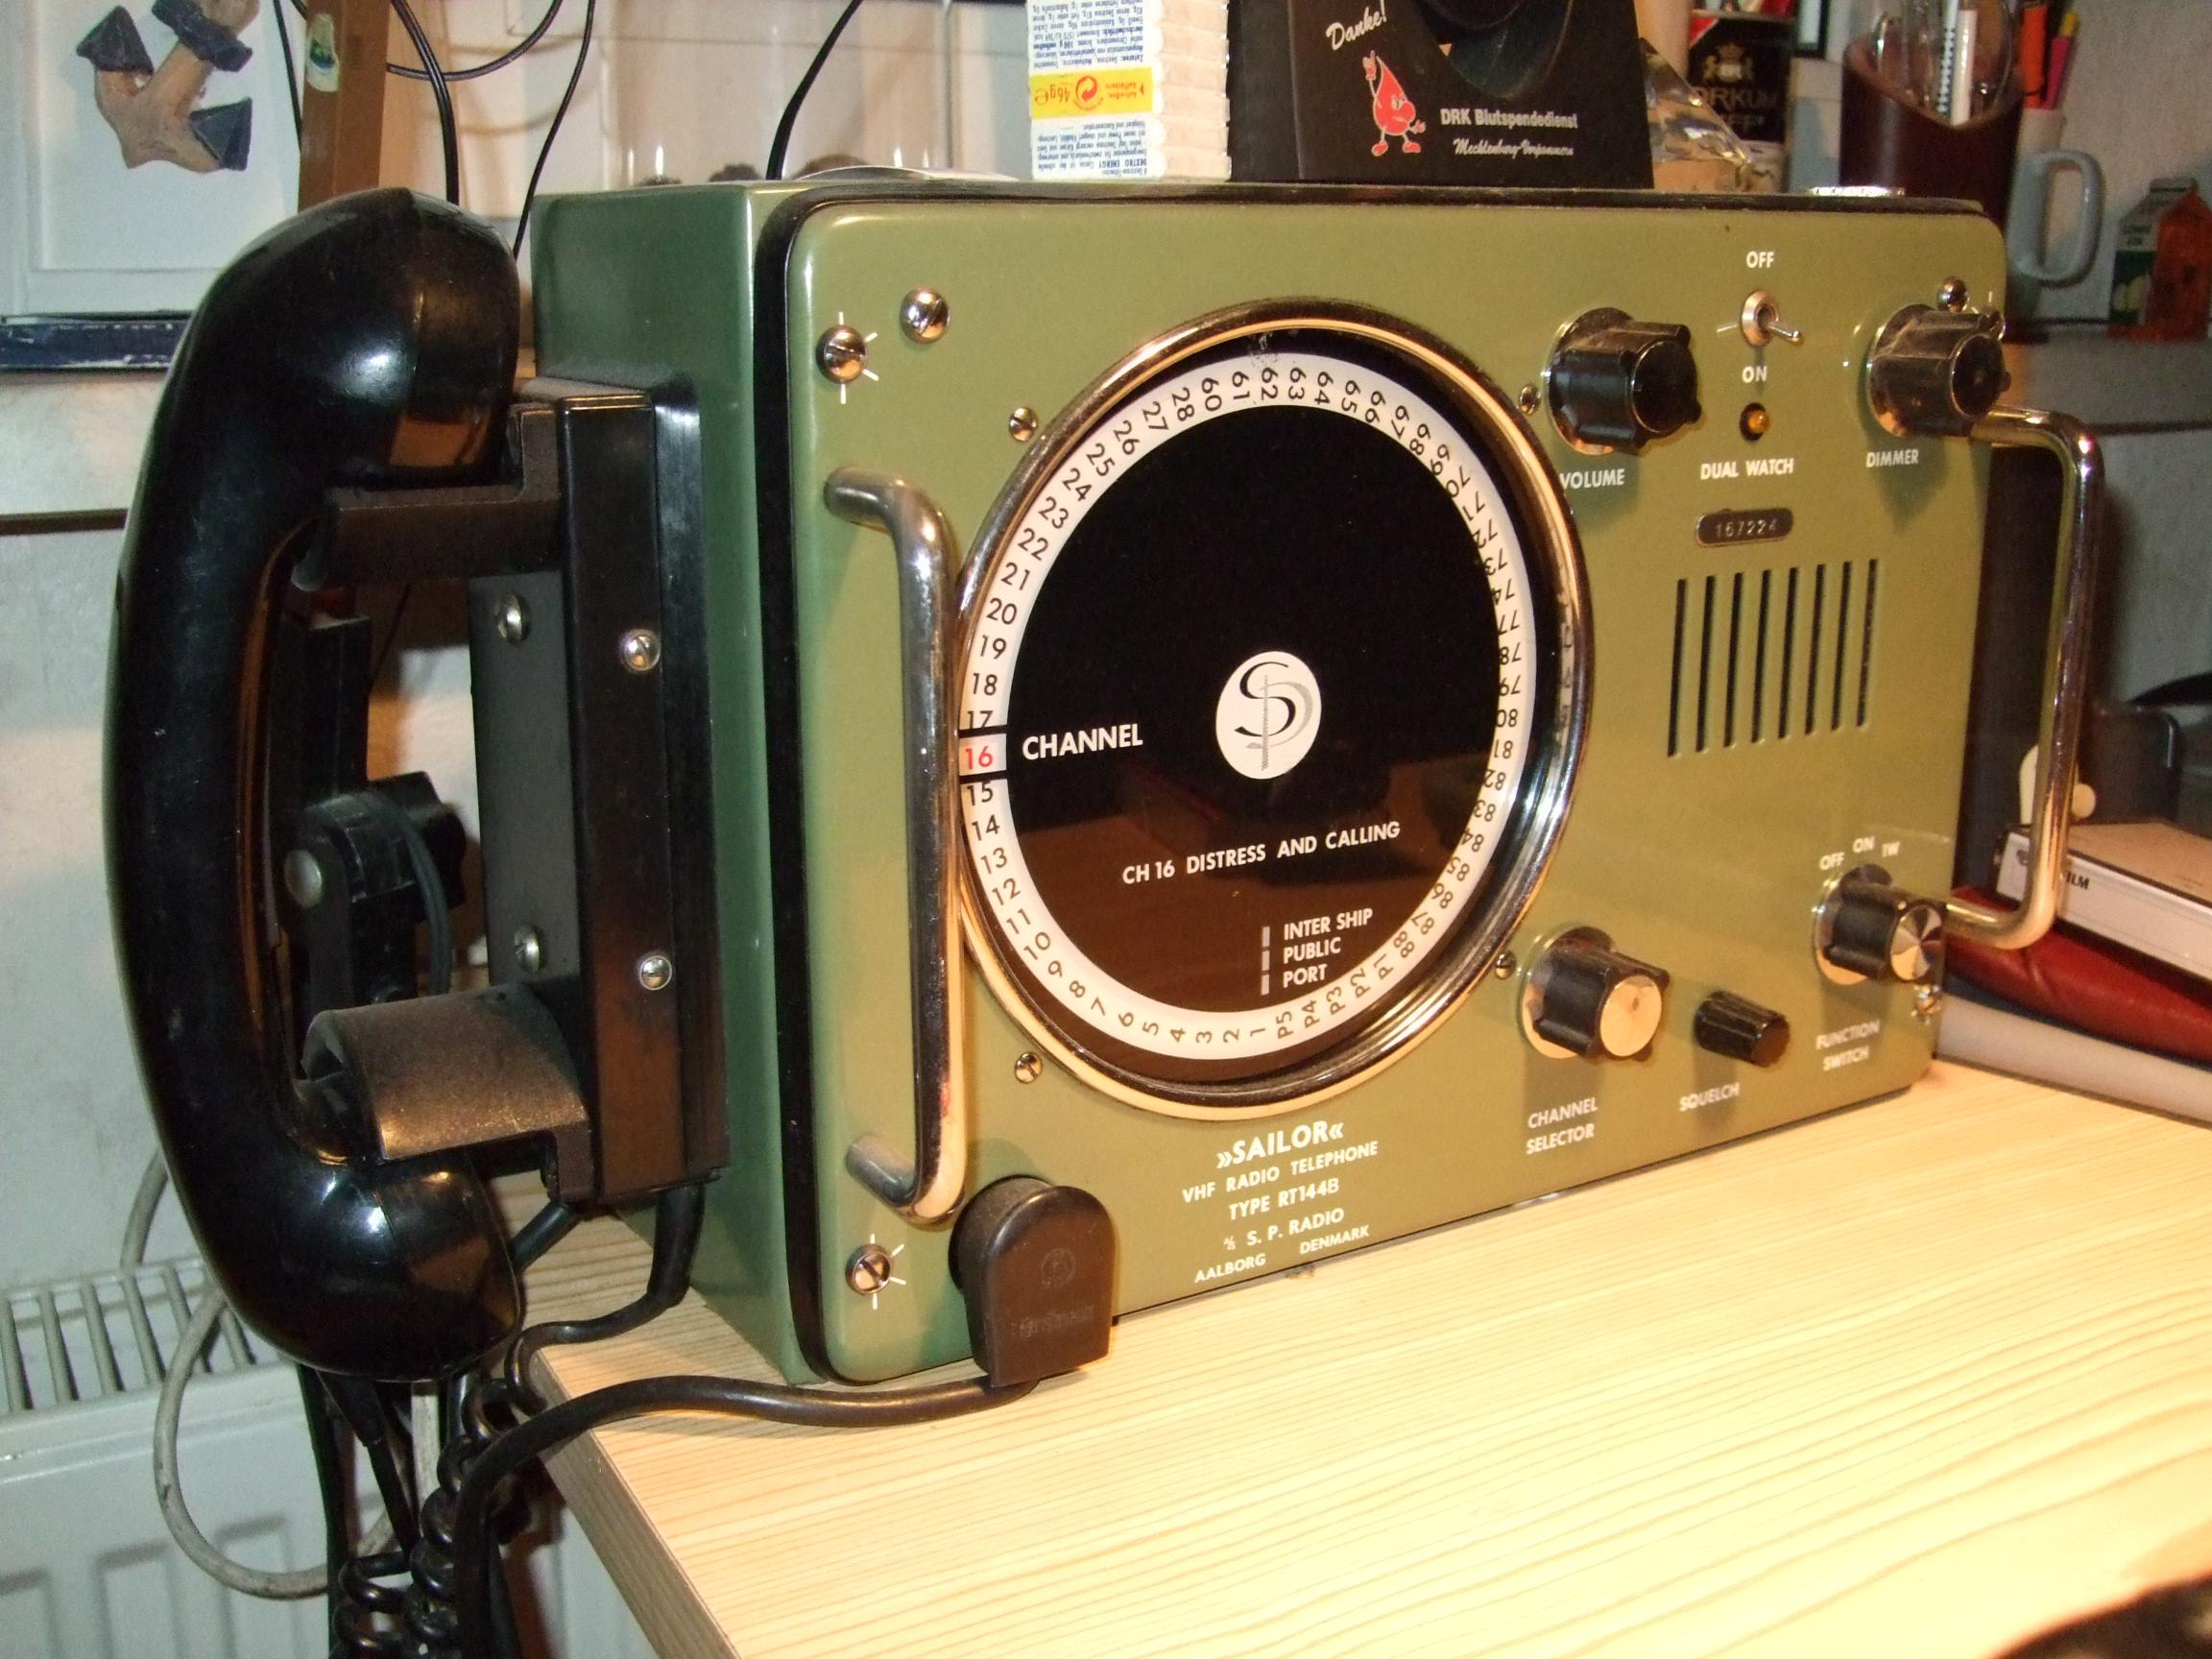
\includegraphics[width=\linewidth]{Figures/RealWorld_Radio.jpg}
    \caption{Real World}
    \label{fig:short-d}
  \end{subfigure}
\end{adjustbox}
  \caption{Domains in the Office-Home dataset \cite{OfficeHome}.}
  \label{fig:domains}
\end{figure}

The experiments were conducted using a ResNet18 convolutional neural network architecture, employing a learning rate of 0.001, a batch size of 128. Image data augmentation techniques were also employed to improve performance of the model, these included random resized crop, color jitter and random grayscale. 


\subsection{Ablation study}
\label{sec:ablation}

The simplified ROS method includes three hyper-parameters that need to be tuned according to the network: the weight assigned to the rotation recognition tasks in stage 1 ($\alpha_1$); the threshold of normality score for considering a target sample as belong to a known category; and the weight assigned to the rotation recognition tasks in stage 2 ($\alpha_2$). The $\alpha_1$ parameter of stage 1 was tuned first. Figure \ref{fig:ClassAcc} shows the class accuracy of stage 1 when trained on the \textit{Art} source domain for a number of epochs and different $\alpha_1$ values, and Figure \ref{fig:RotAcc} shows the corresponding rotation recognition accuracy. As expected the accuracy of both increases with increasing number of epochs, however lower weights take much longer to converge for the rotation recognition tasks. Since the two classifiers are trained simultaneously a balance needs to be sought to reduce over-fitting of either task.

\begin{figure}[!htb]
  \centering
   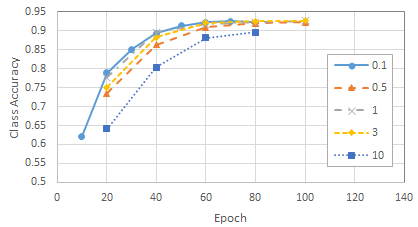
\includegraphics[width=0.95\linewidth]{Figures/ClassAcc.png}
   \caption{Class accuracy during stage 1 training on the Art domain for various weights.}
   \label{fig:ClassAcc}
\end{figure}

\begin{figure}[!htb]
  \centering
   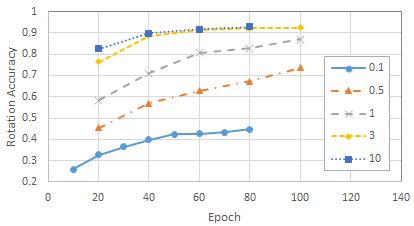
\includegraphics[width=0.95\linewidth]{Figures/RotAcc.png}
   \caption{Rotation recognition accuracy during stage 1 training on the Art domain for various weights.}
   \label{fig:RotAcc}
\end{figure}

The AUC metric was then used to compare the performance of the various weights. The AUC value for the network with \textit{Art} as the source domain and \textit{Clipart} as the target domain is shown in Table \ref{tab:auc}. The highest AUC measured was 0.5578 for a weight of 10 at 40 epochs, therefore 10 was chosen at the values for $\alpha_1$ in stage 1. 

\begin{table}[!htb]
  \centering
  \begin{tabular}{@{}|l|ccccc|@{}}
    \hline
     & \multicolumn{5}{c|}{\textbf{Weight ( $\alpha_1$)}}\\
 \textbf{Epoch} & 0.1 & 0.5 & 1 & 3 & 10 \\
    \hline 
    40 & 0.5293 & 0.4944 & 0.5245 & 0.5492 & 0.5578 \\
   80 & 0.5203 & 0.4873 & 0.5312 & 0.5397 & 0.5548 \\
    \hline
  \end{tabular}
  \caption{AUC for Art -- Clipart}
  \label{tab:auc}
\end{table}

The next step involved tuning the threshold. The threshold should be chosen such that the number of samples recognized as known is similar to the number of samples that are expected to be recognized as known. Considering again the \textit{Art} as source and \textit{Clipart} as target domain combination as an example, the total number of samples in the \textit{Clipart} target domain is 4365, and 3064 of those samples share the same category as those in the \textit{Art} source domain. The model was thus evaluated with different thresholds and the number of samples identified as known analysed. Table \ref{tab:threshold} shows the results of the analysis on the \textit{Art}--\textit{Clipart} domain combination. A threshold of 0.75 results in the number of known samples being most similar to the expected number of known samples of 3064, and so 0.75 was chosen as the threshold for that combination.

\begin{table}[!htb]
  \centering
  \begin{tabular}{@{}|cc|@{}}
    \hline
 \textbf{Threshold} & \textbf{Known Samples} \\
    \hline 
 0.3 & 3778 \\
 0.5 & 3486 \\
 0.7 & 3123 \\
 0.75 & 3019 \\
 0.8 & 2872 \\
    \hline
  \end{tabular}
  \caption{Samples recognised as known for various thresholds for the Art -- Clipart domain combination}
  \label{tab:threshold}
\end{table}

The final step of the ablation study was to tune the stage 2 weight ($\alpha_2$). The evaluation metrics for stage 2 involve the harmonic mean between the accuracy of the known classes and the ability of the classifier to recognize the unknown category, as discussed in \ref{sec:stage2}. The results of stage 2 for the \textit{Art}--\textit{Clipart} domain combination are shown in Table \ref{tab:tuneHOS}. The highest harmonic mean value is 0.4399, for a weight of 3 at 20 epochs.

\begin{table}[!htb]
  \centering
  \begin{tabular}{@{}|ccccc|@{}}
    \hline
 \textbf{Weight ($\alpha_2$}) & \textbf{Epoch} & \textbf{OS$^*$} & \textbf{UNK} & \textbf{HOS} \\
    \hline 
 0.01 & 20 & 0.3026 & 0.5778 & 0.3972 \\
 & 40 & 0.3008 & 0.5743 & 0.3948 \\ \hline
0.1 & 20 & 0.3091 & 0.5896 & 0.4056 \\
 & 40 & 0.3257 & 0.5601 & 0.4119 \\\hline
0.5 & 20 & 0.3280 & 0.5731 & 0.4172 \\
 & 40 & 0.3404 & 0.5495 & 0.4204 \\\hline
3 & 20 & 0.3542 & 0.5802 & 0.4399 \\
 & 40 & 0.3690 & 0.5000 & 0.4246 \\\hline
10 & 20 & 0.3114 & 0.6156 & 0.4136 \\
 & 40 & 0.3367 & 0.5743 & 0.4246 \\
    \hline
  \end{tabular}
  \caption{Stage 2 evaluation metrics for the Art -- Clipart domain combination}
  \label{tab:tuneHOS}
\end{table}

Similar analyses were also conducted for the 11 other possible domain combinations, the results of which can be found in the supplementary material\footnote{Additional results and the complete code is available at \url{https://github.com/DarthReca/AML-Project}.}.


\subsection{Results}

The results for the simplified ROS model for each of the domain combinations is shown in Table \ref{tab:results}. The harmonic mean for each of the different domain combinations lies approximately between 40\% and 55\%. Different combinations performed better than others, however the results were sensitive to the input parameters. Depending on the application, prioritizing the accuracy of the categorization of the known class may prove beneficial and further training would be required.  Results for the complete ROS method were published in \cite{Bucci2020} and reported a harmonic mean between approximately 55\% and 75\%. As expected the complete method performs better than the simplified method adopted in this study, however the simplified method could be employed in situations where a less complex approach is desired.

\begin{table}[!htb]
  \centering
  \begin{tabular}{@{}|ll|ccc|@{}}
    \hline
\multicolumn{2}{|c}{\textbf{Domain}} & & & \\
\textbf{Source} & \textbf{Target} & \textbf{OS$^*$} & \textbf{UNK} & \textbf{HOS} \\ \hline
Art & Clipart & 35.42 & 58.02 & 43.99 \\
& Product & 42.27 & 46.21 & 44.15 \\
 & Real World & 42.50 & 77.01 & 54.77 \\ \hline
Product & Clipart & 38.05 & 55.94 & 45.29 \\
& Art & 33.53 & 46.24 & 38.87 \\
& Real World & 56.50 & 37.72 & 45.24 \\ \hline
Real World & Clipart &43.87 & 50.76 & 47.07 \\
 & Art & 46.86 & 44.54 & 45.67\\
 & Product & 69.44 & 33.95 & 45.60 \\ \hline
Clipart & Real World & 45.46 & 69.06 & 54.83\\
 & Art & 33.71 & 58.14 & 42.67 \\
& Product & 47.75 & 60.02 & 53.19 \\
    \hline
  \end{tabular}
  \caption{Accuracy (\%) for the simplified ROS model on the Office-Home dataset}
  \label{tab:results}
\end{table}


%------------------------------------------------------------------------
\section{Variations}
\label{sec:variations}

Two different variations to the simplified ROS method were also analysed. The first considered the use of alternative self-supervised tasks. The second considered the addition of the center loss to the rotation recognition task.

\subsection{Alternative self-supervised tasks}

The simplified ROS method reported used rotation recognition as the self-supervised task, however many different self-supervised tasks are possible to be employed for use in open-set domain adaptation. This sudy investigated two alternative self-supervised tasks: horizontal flipping; and solving jigsaw puzzles.

\subsubsection*{Horizontal Flipping}

Horizontal flipping is similar to image rotation however instead rotating the image it is flipped along its center y-axis, creating a mirror-image. Horizontal flipping is shown in Figure \ref{fig:horiz}.

\begin{figure}[!htbp]
  \centering
  %\begin{adjustbox}{minipage=\linewidth,scale=0.8}
  \begin{subfigure}[b]{0.4\columnwidth}
    \centering
    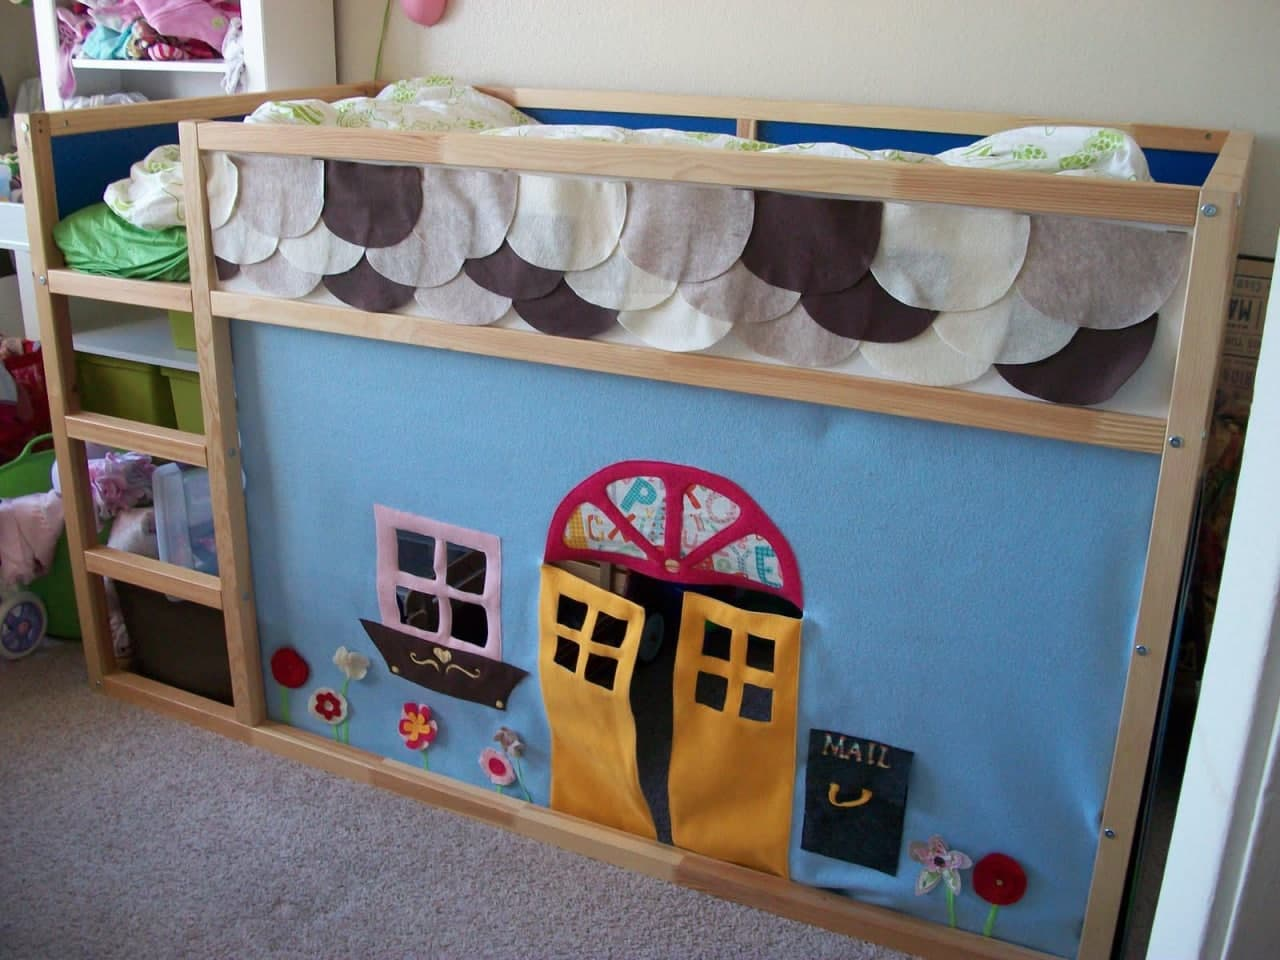
\includegraphics[width=\linewidth]{Figures/FlipRaw.jpg}
    \caption{Raw image}
    \label{fig:short-a}
  \end{subfigure}
\hspace{0.01\textwidth}
  \begin{subfigure}[b]{0.4\columnwidth}
\centering
    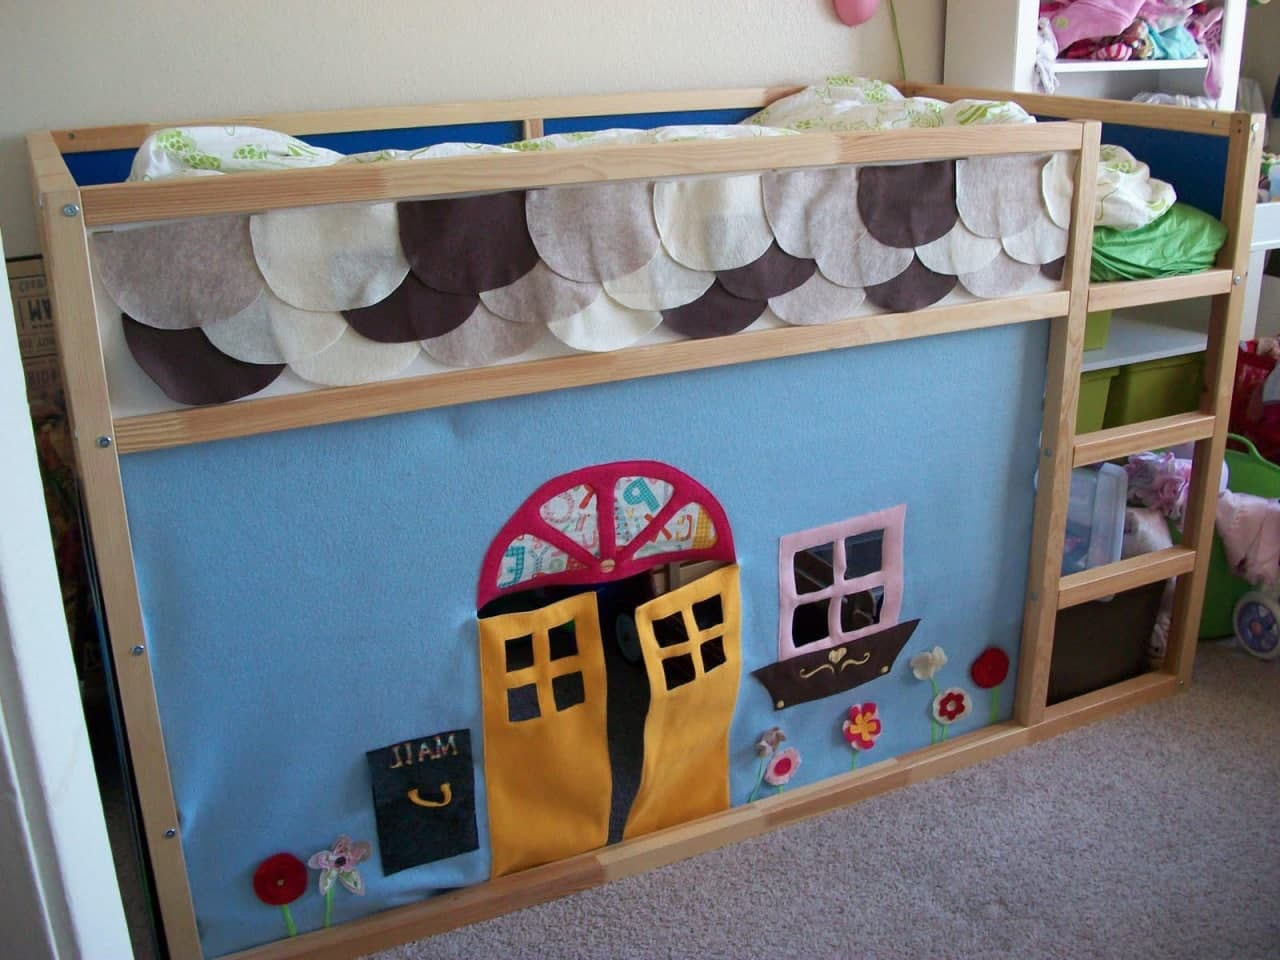
\includegraphics[width=\linewidth]{Figures/FlipHoriz.jpg}
    \caption{Horizontally flipped}
    \label{fig:short-b}
  \end{subfigure}
%\end{adjustbox}
  \caption{Horizontal flipping of an image, adapted from \cite{OfficeHome}.}
  \label{fig:horiz}
\end{figure}

\subsubsection*{Jigsaw Puzzle}

The self-supervised tasks of solving jigsaw puzzles involves being able to recognize an original image given its shuffled parts. The method involves first taking the original image, splitting the image into a number of sections, then creating a set of permutations with a different ordering of those sections. The method can be seen in Figure \ref{fig:jigsaw} as used by \cite{Carlucci2019}. The shuffled images (permutations) are then fed into the convolutional neural network to train the jigsaw classifier alongside the object classifier. This study considered the images broken up into 9 sections, and then recombined based on a random permutation among 30 available permutations. For each image a shuffled one is generated and allocated an index. The convolutional neural network is then trained to predict its index. The Jigsaw puzzle task is formalized as a classification problem over recomposed images with the same dimension of the original one. In this way object recognition and patch reordering can share the same network backbone.

\begin{figure}[!htbp]
  \centering
   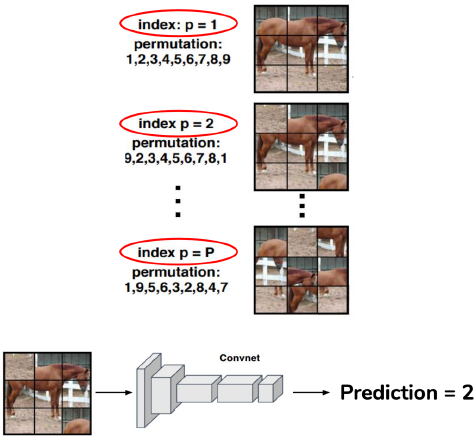
\includegraphics[width=\linewidth]{Figures/Jigsaw2.png}
   \caption{Jigsaw puzzle self-supervised task method, adapted from \cite{Carlucci2019}.}
   \label{fig:jigsaw}
\end{figure}

\subsubsection*{Results}

The harmonic mean results of the simplified ROS method employing different self-supervised tasks for a subset of domain configurations are shown in Table \ref{tab:selfs}. The first two configurations show the best performance using rotation recognition as the self-supervised task, however the third configuration performs best with horizontal flipping. It should be noted that in calculating these results the threshold parameter needed to be tuned independently for each self-supervised task, as this would have a significant effect on the results. The rotation recognition task seems to be the most robust method for conducting open-set domain adaption, in agreeance with the findings from Xu \etal \cite{Xu2019} and Gidaris \etal \cite{Gidaris2018}. As shown by this short study alternative self-supervised tasks may however perform better for some domain configurations.

\begin{table}[!htb]
\small
  \centering
  \begin{tabular}{@{}|ll|ccc|@{}}
    \hline
\multicolumn{2}{|c|}{\textbf{Domain}} & & \textbf{Horizontal} & \textbf{Jigsaw} \\
\textbf{Source} & \textbf{Target} & \textbf{Rotation} & \textbf{Flipping} & \textbf{Puzzle} \\ \hline
Art & Clipart & 43.99 & 35.11 & 18.64 \\
Product & Art & 38.87 & 25.01 & 36.17\\
Real World & Product  & 45.60 & 53.58 & 49.46\\
    \hline
  \end{tabular}
  \caption{Harmonic mean (\%) for the simplified ROS model with different self-supervised tasks on the Office-Home dataset}
  \label{tab:selfs}
\end{table}


\subsection{Center Loss}

The center loss was introduced by Wen \etal \cite{Wen2016} as an additional objective function for enhancing the discriminative power of learned deep features. It involves learning the center of the deep features for each class, prioritizing features that are close to the center and adding a penalty to the distance between the deep features and their corresponding centers \cite{Wen2016}. The center loss function is optimized alongside the soft max loss, with the two losses jointly supervised. A hyper-parameter is introduced representing the weight of the center loss contribution, and is tuned to balance the two loss functions. The difference between the features learned by a classifier training with the soft max loss function on the MNIST dataset \cite{MNIST}, compared with the inclusion of the center loss during training is shown in Figure \ref{fig:centerloss}. The features learned with the inclusion of center loss can clearly be seen to provide greater discriminative power.

\begin{figure}[!htbp]
  \centering
  %\begin{adjustbox}{minipage=\linewidth,scale=0.8}
  \begin{subfigure}[b]{0.45\columnwidth}
    \centering
    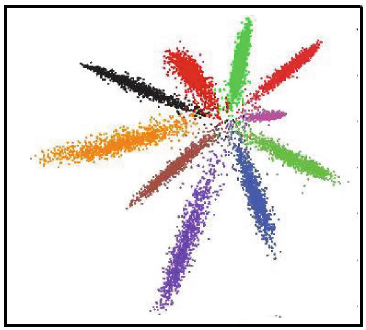
\includegraphics[width=\linewidth]{Figures/SoftMaxLoss.png}
    \caption{Soft Max Loss}
    \label{fig:short-a}
  \end{subfigure}
  \hfill
  \begin{subfigure}[b]{0.45\columnwidth}
\centering
    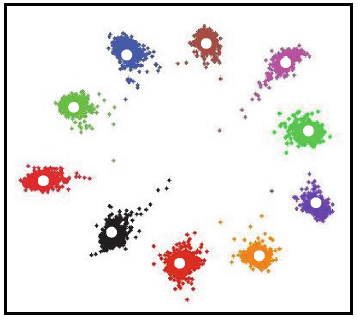
\includegraphics[width=\linewidth]{Figures/CenterLoss.png}
    \caption{Center Loss}
    \label{fig:short-b}
  \end{subfigure}
%\end{adjustbox}
  \caption{Comparison of features learned when including the center loss on the MNIST dataset, adapted from \cite{Wen2016}.}
  \label{fig:centerloss}
\end{figure}

The center loss has been implemented during the first step of the model, and used to understand the effect of this loss on the separation phase.

\subsubsection*{Results}

An ablation study was performed to select the most appropriate weight ($\alpha_w$) of the center loss contribution. The initial weights considered were based on those reported by Bucci \etal \cite{Bucci2020} in their research on the Office-Home \cite{OfficeHome} and Office31 datasets \cite{Office31}. High values of $\alpha_w$ were found to give too much importance to the center loss at the expense of the soft max loss, and the model converged extremely slowly. For this reason the results analysed here consider only weight values lower or equal to $0.01$.

Table \ref{tab:center_loss} shows a comparison of the AUC values with and without the introduction of center loss, with $\alpha_1 = 10$ trained for 40 epochs. The inclusion of center loss was able to improve the accuracy for all domain configurations considered. It also improved the AUC metric for the second two domain configurations, however was detrimental in the first configuration. Due to the similarity of the results presented in \ref{tab:center_loss} the findings are inconclusive, and further investigations would be necessary to understand if the center loss could be used effectively in this scenario.

\begin{table}[!htbp]
	\centering
	\small
	\begin{tabular}{|l|c|c|c|c|}
		\hline
		 & & & \multicolumn{2}{c|}{\textbf{Weight  $\alpha_w$}} \\
		Domains & Metric & Standard & 0.001 & 0.01\\
		\hline
		\multirow{2}{*}{Art $\to$ Clipart}
		& AUC & \textbf{0.5590} & 0.5486 & 0.5302\\ 
		& Accuracy & 0.8988 & 0.9150 & 0.9150\\
		\hline
		\multirow{2}{*}{Product $\to$ Art}
		& AUC & 0.4997 & \textbf{0.5077} & 0.5023\\ 
		& Accuracy & 0.9513 & 0.9612 & 0.9631\\
		\hline
		\multirow{2}{*}{Art $\to$ RealWorld}
		& AUC & 0.4956 & \textbf{0.5000} & 0.4967\\ 
		& Accuracy & 0.8988 & 0.9128 & 0.9139\\
		\hline
	\end{tabular}
	\caption{Comparison of center loss model with standard model}
	\label{tab:center_loss}
\end{table}


%------------------------------------------------------------------------
\section{Conclusions}
\label{sec:conclusion}

This study investigated the use of a simplified ROS method for conducting open-set domain adaptation. The method was a simplified version of the ROS method reported in \cite{Bucci2020} by removing the center loss and using only a single-head rotation classifier. Results of the simplified version performed worse than the complete version when comparing the harmonic mean between the accuracy of the classification of known categories and the accuracy of identifying the unknown class. The simplified method however could be improved with further investigation into the effect of different input parameters, and could prove beneficial in situations where a less complex approach is desired. 

Variations to the simplified ROS method were also investigated, including the use of alternative self-supervised tasks and the addition of the center loss to the training of stage 1 of the model. Rotation recognition was found to be the most robust method for conducting self-supervision, however the alternative techniques could perform well in specific scenarios.  The addition of the center loss to stage 1 in some instances was able to improve the performance of the model, and increase the pace at which appropriate features were identified. Further investigation into the utility of center loss is however recommended to better understand its application to open-set domain adaptation problems.


\subsection{Acknowledgements}
The authors would like to thank Silvia Bucci for her assistance and guidance in completing this study.


%%%%%%%%% REFERENCES
{\small
\bibliographystyle{ieee_fullname}
\bibliography{egbib}
}

\end{document}
